\documentclass[11pt,a4paper]{article}
\usepackage[T1]{fontenc}
\usepackage[utf8]{inputenc}
\usepackage{mathpazo}
\usepackage[a4paper,margin=25mm,headheight=15pt]{geometry}
\usepackage{amsmath,amssymb,amsthm,mathtools}
\usepackage{microtype,booktabs,longtable,tabularx,array,graphicx}
\usepackage{xcolor,enumitem,fancyhdr,titlesec,float}
\usepackage[breaklinks=true,colorlinks=true,linkcolor=navy,citecolor=teal,urlcolor=teal]{hyperref}
\definecolor{navy}{HTML}{16324F}
\definecolor{teal}{HTML}{087E8B}
\definecolor{light}{HTML}{F0F5F8}
\titleformat{\section}{\large\bfseries\color{navy}}{\thesection}{0.7em}{}
\titleformat{\subsection}{\normalsize\bfseries\color{navy}}{\thesubsection}{0.7em}{}
\pagestyle{fancy}
\fancyhf{}
\fancyhead[L]{\small Uniform exponential-tilting guarantees}
\fancyhead[R]{\small 8 October 2026}
\fancyfoot[C]{\thepage}
\setlength{\parskip}{0.35em}
\setlength{\parindent}{1.25em}
\setlength{\emergencystretch}{2em}
\setlist{itemsep=0.25em,topsep=0.35em}
\newtheorem{theorem}{Theorem}[section]
\newtheorem{lemma}[theorem]{Lemma}
\newtheorem{corollary}[theorem]{Corollary}
\newtheorem{proposition}[theorem]{Proposition}
\theoremstyle{definition}
\newtheorem{definition}[theorem]{Definition}
\newtheorem{remark}[theorem]{Remark}
\newcommand{\E}{\mathbb E}
\newcommand{\Prob}{\mathbb P}
\newcommand{\Var}{\operatorname{Var}}
\newcommand{\ii}{\mathrm i}
\newcommand{\ee}{\mathrm e}
\newcommand{\R}{\mathbb R}
\newcommand{\Z}{\mathbb Z}
\newcommand{\supp}{\operatorname{supp}}
\newcommand{\ceil}[1]{\left\lceil #1\right\rceil}
\newcommand{\floor}[1]{\left\lfloor #1\right\rfloor}
\newcommand{\abs}[1]{\left|#1\right|}
\newcommand{\norm}[1]{\left\|#1\right\|}
\newcommand{\code}[1]{\texttt{\detokenize{#1}}}
\newcommand{\BigO}{\mathcal O}
\newcommand{\inputifexists}[1]{\IfFileExists{#1}{\input{#1}}{\textit{The accompanying reproducibility script generates this table.}}}
\hypersetup{pdftitle={Uniform Exponential-Tilting Guarantees for Coefficients and Constrained Sampling},pdfauthor={ChatGPT; prepared for Vladimir Reshetnikov},pdfsubject={Certified sparse Fourier algorithms and exact sampling of two-row contingency tables}}
\begin{document}
\hypersetup{pageanchor=false}
\begin{titlepage}
\centering
\vspace*{16mm}
{\small\bfseries\color{teal} RESEARCH ARTICLE AND REPRODUCIBLE ARTIFACTS\par}
\vspace{12mm}
{\Huge\bfseries\color{navy} Uniform Exponential-Tilting Guarantees\par}
\vspace{6mm}
{\LARGE for Coefficients and Constrained Sampling\par}
\vspace{11mm}
{\large Certified sparse Fourier extraction and exact sampling\par}
{\large of two-row contingency tables with arbitrary margins\par}
\vspace{18mm}
{\large Prepared for Vladimir Reshetnikov\par}
{\normalsize ChatGPT research collaboration\par}
\vspace{5mm}
{8 October 2026\par}
\vfill
\begin{minipage}{0.88\textwidth}
\small
\textbf{Principal results.} A specified coefficient of a product of positive linear factors admits a deterministic relative approximation using only $\BigO(\log(1/\varepsilon))$ Fourier evaluations after coarse exponential tilting. The construction handles binary-encoded multiplicities and computes all representative conditional inclusion probabilities to additive accuracy at the same order of work. A second theorem gives an explicit $5\sqrt n$ bound on the expected number of proposals in a tilted exact sampler for every feasible two-row contingency table, with no equality or comparability assumption on its margins.

\textbf{Research status.} The article provides complete proofs of its mathematical guarantees and executable checks. Its contribution is a quantitative strengthening and synthesis of established methods. The exact uniform guarantees were not located in the primary sources surveyed here; this is a scoped literature assessment, rather than a claim that a named longstanding open problem has been resolved.
\end{minipage}
\vspace*{12mm}
\end{titlepage}
\hypersetup{pageanchor=true}
\pagenumbering{roman}

\begin{abstract}
Exponential tilting makes a prescribed coefficient into a central probability, but a useful algorithm also needs uniform control of the resulting central atom, Fourier aliases, numerical cancellation, and parameter-selection cost. We give such control for Poisson--binomial distributions. If an integer $k$ is within $1/4$ of the mean and the variance is $V$, a roots-of-unity quadrature of modulus $M=\min\{N+1,\lceil2\sqrt{VL}+2L\rceil\}$, with $L=\log(1000/\varepsilon)$, requires only $\BigO(L)$ retained frequencies and approximates $\Prob(S=k)$ to relative error at most $\varepsilon$. The guarantee is uniform in $N$, the Bernoulli parameters, the variance, and the rarity of the original untilted coefficient. Prefix and suffix products reuse the same frequencies for all conditional inclusion marginals. For a succinct product with multiplicities $m_i$ and degree $N=\sum_i m_i$, the Fourier work is $\BigO(L\sum_i\log(m_i+1))$ elementary arithmetic operations. A bisection--Newton argument bounds coarse-tilt preprocessing by $\BigO(s[\log(2+W)+\log\log(N+2)])$, where $s$ is the number of groups and $W$ is the spread of their log odds. Explicit interval enclosures separate analytic error from roundoff.

The same entropy estimate yields a second result for bounded integer compositions. Common truncated-geometric tilting and one deterministically completed coordinate give exact uniform samples of arbitrary two-row contingency tables in at most $5\sqrt n$ expected proposals at exact centering, or $5e\sqrt n$ at an explicitly constructible rational tilt. The bound strengthens the equal-margin asymptotic proposal estimate in the inspected DeSalvo--Zhao preprint. We prove a sharper instance-dependent bound, a polynomial-bit implementation theorem, and the sharpness of the order $\sqrt n$ within this proposal family. Reproducible ball-arithmetic coefficient calculations, exact rational sampling checks, and further research questions accompany the proofs.
\end{abstract}

\setcounter{tocdepth}{1}
\tableofcontents
\clearpage
\pagenumbering{arabic}

\section{Research objective, provenance, and precise scope}

The starting point was the \emph{openai/math} manuscript collection, in particular its themes of Fourier arithmetic and sampling with unrestricted margins \cite{openai}. Those themes suggest a concrete algorithmic question: when a task asks for one coefficient or one constrained sample, which parts of a full distribution calculation can be avoided, and which estimates make the saving rigorous? The repository's README explicitly distinguishes stages of verification. No unverified headline theorem from that collection is assumed anywhere below. The results here follow from elementary probability, log-concavity, complex Fourier inversion, and explicit algorithms whose proofs are supplied.

The paper develops two related improvements. The first strengthens Fourier approximation from an absolute-error description to a uniform relative guarantee for a prescribed Poisson--binomial atom, including extremely rare original atoms and succinct input. The second turns a central-probability lower bound into a proposal bound for exact sampling that holds uniformly over every pair of row sums and every vector of column sums.

\subsection{What the first algorithm computes}

Let
\begin{equation}\label{eq:polynomial}
 P(z)=\prod_{i=1}^{s}(a_i+b_i z)^{m_i},\qquad
 a_i,b_i>0,\quad m_i\in\Z_{\ge1},\quad N=\sum_i m_i.
\end{equation}
Given an integer $0\le k\le N$ and $0<\varepsilon\le1/2$, the main task is to approximate
$c_k=[z^k]P(z)$ with $\abs{\widehat c_k/c_k-1}\le\varepsilon$.
The multiplicities may be encoded in binary. The ordinary input model is recovered by taking $m_i=1$ and $s=N$.

For a Bernoulli sum, set $a_i=1-p_i$ and $b_i=p_i$; then $c_k$ is exactly a probability. For weighted $k$-subsets, set $a_i=1$ and $b_i=w_i$; then $c_k$ is an elementary symmetric coefficient, or its grouped analogue. The conditional probability that a particular trial in group $i$ equals one is another output. We guarantee additive accuracy for these marginals. Multiplying a representative marginal by $m_i$ gives an expected group count, whose additive error is correspondingly multiplied by $m_i$.

Zero coefficients of individual factors are handled first: a factor with $b_i=0$ contributes a constant, and a factor with $a_i=0$ contributes a known monomial and an index shift. A zero polynomial and infeasible target indices are recognized exactly. The cases $k=0,N$ are simple products and need no Fourier inversion.

\subsection{What is strengthened relative to prior work}

Several ingredients have substantial prior literature. Exponential shifting for accurate rare Poisson--binomial tails is explicit in Peres--Lee--Keich \cite{plk}; their full-distribution convolution has arithmetic cost $\BigO(N(\log N)^2)$ and their discussion identifies rigorous cumulative numerical-error bounds as a further objective. Diakonikolas--Kane--Stewart \cite{dks} establish approximately sparse Fourier representations for sums of independent integer random variables; for Bernoulli sums the effective frequency count has logarithmic accuracy dependence. Their setting is learning and total-variation approximation. Bornemann \cite{bornemann} studies accurate coefficient extraction through optimized Cauchy integrals. Wilson--Keich \cite{wk2017,wk2016} give rigorous accuracy results for related FFT computations.

Our specific first contribution is a finite-accuracy theorem combining these ideas with \emph{local relative alias control}, a mean-centering tolerance that is fixed rather than asymptotically vanishing, a full small-variance branch, simultaneous marginal calculations, and support for binary multiplicities. Neither tilting nor Fourier sparsity is claimed as new. A single requested coefficient and a complete distribution are different output tasks; their operation counts must be compared with that distinction visible.

For the second result, Dyer--Greenhill \cite{dg} give a heat-bath chain with mixing time quadratic in the number of columns and logarithmic in the table sum. Kijima--Matsui \cite{km} give polynomial-time perfect sampling. DeSalvo--Zhao \cite{dz} develop probabilistic divide-and-conquer (PDC); Algorithm 3 and Theorem 2.10 of the inspected arXiv version give a particularly simple exact two-row sampler. Its Corollary 2.11 obtains a $\BigO(\sqrt n)$ rejection estimate under equal row sums and equal column sums. We prove a uniform nonasymptotic bound after common exponential tilting, without those restrictions. We refer specifically to arXiv:1507.00070v4 for the inspected theorem numbering.

\begin{center}
\small
\begin{tabularx}{\textwidth}{@{}p{0.21\textwidth}XX@{}}
\toprule
Method or result & Output and established feature & Guarantee developed here \\
\midrule
Shifted FFT convolution \cite{plk} & Full shifted law; practical relative accuracy for rare tails & Certified relative accuracy for one mass with $\BigO(\log(1/\varepsilon))$ retained frequencies \\
Sparse Fourier learning \cite{dks} & Approximate Fourier support; additive/TV approximation & Relative pointwise error after coarse tilt, including very small variance \\
Cauchy coefficient extraction \cite{bornemann} & Contour choice and numerical conditioning & Uniform bounds for this product class and binary multiplicities \\
Two-row PDC \cite{dz} & Exactness; equal-margin asymptotic proposal estimate & At most $5\sqrt n$ expected proposals at centering for every feasible margin vector \\
\bottomrule
\end{tabularx}
\end{center}

\subsection{Computational models}

An \emph{elementary arithmetic operation} below includes real or complex arithmetic and a call to $\exp$, $\log$, or a trigonometric function at the specified precision. Integer powers are implemented by repeated squaring and their multiplication cost is counted. This convention is explicit because a bound on product evaluations alone is not a bit-complexity theorem.

For the coefficient problem we state the coarse-tilt cost and Fourier cost separately, then give numerical conditioning and conservative precision requirements. The delivered coefficient implementation uses Arb/Acb balls through python-flint. For the table sampler, the exact fair-random-bit model is treated separately from the number of proposals. The delivered rational reference sampler enumerates individual finite supports; the proof of the polynomial-bit sampler specifies a different, lazy interval implementation. These implementation scopes are part of the results.

\section{A central atom from log-concavity and entropy}\label{sec:entropy}

A finite integer probability mass function $p_j$ is \emph{log-concave with no gaps} if its positive support is an integer interval and $p_j^2\ge p_{j-1}p_{j+1}$. Its log probabilities have a concave piecewise-linear interpolation on that interval.

\begin{lemma}[Preservation under convolution]\label{lem:convolution}
The convolution of two finite log-concave integer mass functions with no gaps has the same properties. In particular, this applies to sums of independent Bernoulli variables and to sums of independent truncated geometric variables.
\end{lemma}
\begin{proof}
For a sequence $a$, form its Toeplitz matrix $A_{ij}=a_{i-j}$. Monotonicity of the consecutive ratios of a gap-free log-concave sequence implies that every order-two minor of $A$ is nonnegative: the product of the two entries with closer indices is at least the product of the two with more separated indices. The same holds for the matrix $B$ of a second sequence. The order-two Cauchy--Binet identity makes every order-two minor of $AB$ a sum of products of nonnegative minors. Its entries are $(a*b)_{i-j}$. The adjacent minors give log-concavity of $a*b$, and the sum of the two support intervals has no gaps. All sums involved in each minor are finite. Bernoulli masses and the sequences proportional to $1,q,\ldots,q^c$ satisfy the hypotheses.
\end{proof}

\begin{lemma}[Integer mean]\label{lem:integermean}
If $Y$ has a finite gap-free log-concave mass function, integer mean $k$, and variance $v$, then
\begin{equation}\label{eq:centralentropy}
 \Prob(Y=k)\ge\ee^{-H(Y)}\ge
 \frac{1}{\sqrt{2\pi\ee\,(v+1/12)}}.
\end{equation}
Here entropy uses natural logarithms.
\end{lemma}
\begin{proof}
Let $g$ be the concave interpolation of $\log p_j$. Jensen gives
$g(k)=g(\E Y)\ge\E g(Y)=\sum_jp_j\log p_j=-H(Y)$.
For an independent $U$ uniform on $(-1/2,1/2)$, the density of $Y+U$ equals $p_j$ on the unit interval centered at $j$. Thus its differential entropy is $H(Y)$ and its variance is $v+1/12$. The Gaussian entropy bound gives
$H(Y)\le\tfrac12\log(2\pi\ee(v+1/12))$.
For completeness, that bound follows by applying nonnegativity of relative entropy to the density of $Y+U$ and the Gaussian with the same mean and variance, then evaluating the Gaussian logarithm. Exponentiation proves the result.
\end{proof}

The exact mean-centering parameter usually is not a rational input. The following robust version removes any need to compute it exactly.

\begin{lemma}[Coarse mean centering]\label{lem:coarsemean}
Under the same log-concavity hypotheses, if $\abs{\E Y-k}\le1/4$, then
\begin{equation}\label{eq:coarselower}
 \Prob(Y=k)\ge3^{-1/4}\ee^{-H(Y)}
 \ge \frac{1}{6\sqrt{v+1}}.
\end{equation}
\end{lemma}
\begin{proof}
Write $\E Y=k+d$ with $0\le d\le1/4$; reflection handles negative $d$. If $p_{k+1}\le p_k$, then $g(k+d)\le g(k)$ and Jensen proves the stronger integer-mean entropy bound. Otherwise let $R=p_{k+1}/p_k>1$. Log-concavity implies $p_{j-1}\le p_j/R$ for $j\le k+1$. If $F$ is the distribution function, summation yields
$F(k+1-m)\le R^{-m}$ for every $m\ge1$. Hence
\[
 \E Y\ge k+1-\E[(k+1-Y)_+]
 =k+1-\sum_{m\ge1}F(k+1-m)
 \ge k+1-\frac{1}{R-1}.
\]
It follows that $R\le1+(1-d)^{-1}\le7/3<3$. Therefore
$g(k+d)-g(k)=d\log R\le\tfrac14\log3$.
Combine this with $g(k+d)\ge-H(Y)$ and Lemma~\ref{lem:integermean}'s entropy argument. Finally
$3^{1/4}\sqrt{2\pi\ee(v+1/12)}\le6\sqrt{v+1}$.
The target $k$ lies in the support, since the mean is inside a gap-free integer interval and is within $1/4$ of $k$.
\end{proof}

The value of these estimates is their uniformity. They require neither a local central limit theorem nor a lower bound on variance. For example, a law concentrated almost entirely at one integer is fully covered.

\section{Tilting a coefficient into a central probability}\label{sec:tilt}

For a real parameter $\theta$, put
\begin{equation}\label{eq:tiltedq}
 q_i(\theta)=\frac{b_i\ee^\theta}{a_i+b_i\ee^\theta},\quad
 \mu(\theta)=\sum_i m_iq_i(\theta),\quad
 V(\theta)=\sum_i m_iq_i(\theta)(1-q_i(\theta)).
\end{equation}
Let $S_\theta$ be the sum of the corresponding independent Bernoulli trials, conceptually expanded according to their multiplicities. Coefficient comparison gives the exact identity
\begin{equation}\label{eq:untilt}
 c_k=\exp\{\Lambda(\theta)\}\,\Prob(S_\theta=k),\qquad
 \Lambda(\theta)=\sum_i m_i\log(a_i+b_i\ee^\theta)-k\theta.
\end{equation}
It holds for \emph{every} real $\theta$. Using an approximate saddle introduces no extra approximation into this identity; it merely changes the distribution whose central atom is evaluated.

For $0<k<N$, the continuous increasing function $\mu$ goes from $0$ to $N$, so a unique exact centering point $\theta_*$ exists. We need only a point with $\abs{\mu(\theta)-k}\le1/4$.

\begin{lemma}[Differential control]\label{lem:logvariance}
For the positive factors in \eqref{eq:polynomial},
\[
 \mu'(\theta)=V(\theta)>0,\qquad
 \abs{V'(\theta)}\le V(\theta),\qquad
 0<V(\theta)\le N/4.
\]
Consequently $\ee^{-\abs{u}}V(\theta)\le V(\theta+u)\le\ee^{\abs{u}}V(\theta)$.
\end{lemma}
\begin{proof}
Differentiate $q_i'=q_i(1-q_i)$. This gives
$V'=\sum_i m_iq_i(1-q_i)(1-2q_i)$, whose absolute value is at most $V$. Integrate the bound on $(\log V)'$; the remaining claims follow term by term.
\end{proof}

\begin{theorem}[Fast coarse-tilt preprocessing]\label{thm:newton}
Let $\rho_i=\log(b_i/a_i)$ and $W=\max_i\rho_i-\min_i\rho_i$. A parameter satisfying $\abs{\mu(\theta)-k}\le1/4$ can be found in
\begin{equation}\label{eq:tiltcost}
 \BigO\!\left(s\,[1+\log(2+W)+\log\log(N+2)]\right)
\end{equation}
elementary arithmetic operations, in exact real arithmetic.
\end{theorem}
\begin{proof}
A bracket for $\theta_*$ is
\[
 \theta_-=-\max_i\rho_i-\log(2N),\qquad
 \theta_+=-\min_i\rho_i+\log(2N).
\]
At the lower endpoint every $q_i<1/(2N)$, so $\mu<1/2<k$. At the upper endpoint $\mu>N-1/2>k$. Bisect until the bracket width is at most one. Its midpoint satisfies $\abs{\theta-\theta_*}\le1/2$, and the number of bisections is
$\BigO(1+\log(W+2\log(2N)))$.

Now apply Newton's update
\[
 \theta_{t+1}=\theta_t-\frac{\mu(\theta_t)-k}{V(\theta_t)}.
\]
Let $e_t=\theta_t-\theta_*$. Express the numerator as an integral of $V$ between $\theta_*$ and $\theta_t$ and apply Lemma~\ref{lem:logvariance}. In either sign of $e_t$,
\[
 \abs{e_{t+1}}\le\int_0^{\abs{e_t}}(\ee^u-1)\,du
 =\ee^{\abs{e_t}}-1-\abs{e_t}\le\abs{e_t}^2
 \quad(\abs{e_t}\le1/2).
\]
Thus $\abs{e_t}\le2^{-2^t}$. After
$t=\lceil\log_2(\max\{1,\log_2N\})\rceil$ updates, $\abs{e_t}\le1/N$, and the derivative bound $\mu'\le N/4$ gives the required mean tolerance. Each mean--variance evaluation costs $\BigO(s)$. Combining the counts proves \eqref{eq:tiltcost}.
\end{proof}

This theorem counts the tilt rather than treating it as an oracle. A certified bisection search initialized with the translated bracket above has the conservative evaluation bound
$\BigO(s[1+\log(N(2+W))])$ and can stop as soon as the $1/4$ residual is proved. The delivered code instead starts at zero and doubles an absolute-distance bracket, so its count also depends on the location of the log odds. Writing $R=\max_i\abs{\rho_i}$, that strategy uses
$\BigO(s[1+\log(N+2)+\log(2+R+\log(N+2))])$
mean-evaluation work at sufficient precision. These bounds distinguish two different bracket initializations. Safeguarded interval Newton updates can realize the faster theorem's structure, but their finite-precision stopping logic must be checked explicitly.

\section{Local bounds for a Bernoulli sum}\label{sec:local}

For the next two sections fix a Bernoulli sum $S$, with variance $V>0$ and $\abs{\mu-k}\le1/4$. Multiplicities are immaterial to the probability proofs. Define its centered characteristic function
\begin{equation}\label{eq:char}
 f(t)=\E\ee^{\ii t(S-k)}
 =\ee^{-\ii kt}\prod_i(1-q_i+q_i\ee^{\ii t})^{m_i}.
\end{equation}

\begin{lemma}[Fourier envelope and maximal atom]\label{lem:envelope}
For $-\pi\le t\le\pi$,
\begin{equation}\label{eq:envelope}
 \abs{f(t)}\le\exp\{-2V\sin^2(t/2)\}.
\end{equation}
Any Bernoulli sum of variance $v$ has maximal point mass at most
$\sqrt2/\sqrt{v+1}$.
\end{lemma}
\begin{proof}
The squared modulus of one factor is
$1-4q_i(1-q_i)\sin^2(t/2)$.
Use $\sqrt{1-x}\le\ee^{-x/2}$ and multiply. Fourier inversion bounds every atom by $(2\pi)^{-1}\int_{-\pi}^{\pi}\abs{f(t)}dt$. Since $\sin(\abs t/2)\ge\abs t/\pi$, the Gaussian integral gives a bound $\sqrt{\pi/(8v)}$ when $v>0$. Combine it with the trivial bound one: for $v\le1$ use one, and for $v\ge1$ use the Gaussian bound. Both are at most $\sqrt2/\sqrt{v+1}$.
\end{proof}

\begin{lemma}[Local Chernoff estimate]\label{lem:localchernoff}
For every nonzero integer $r$,
\begin{align}
 \Prob(S=k+r)
 &\le \frac{\sqrt2\,\ee^{3/4}}{\sqrt{V+1}}
 \exp\!\left[-\min\left\{\frac{r^2}{4V},\frac{\abs r}{2}\right\}\right],
 \label{eq:abslocal}\\
 \frac{\Prob(S=k+r)}{\Prob(S=k)}
 &\le20\exp\!\left[-\min\left\{\frac{r^2}{4V},\frac{\abs r}{2}\right\}\right].
 \label{eq:rellocal}
\end{align}
\end{lemma}
\begin{proof}
Let $K(\alpha)=\log\E\ee^{\alpha S}$ and tilt the law once more by $\alpha$. For $\abs\alpha\le1$, Lemma~\ref{lem:logvariance} gives $V_\alpha\ge\ee^{-1}V$ and
\[
 K(\alpha)-\mu\alpha
 \le V(\ee^{\abs\alpha}-1-\abs\alpha)\le V\alpha^2.
\]
At an integer $k+r$, tilting and Lemma~\ref{lem:envelope} imply
\[
 \Prob(S=k+r)
 \le\frac{\sqrt{2\ee}}{\sqrt{V+1}}
 \exp\{V\alpha^2-\alpha r+\alpha(\mu-k)\}.
\]
Choose $\alpha=\operatorname{sgn}(r)\min\{\abs r/(2V),1\}$. The first two exponent terms are at most $-r^2/(4V)$ when $\abs r\le2V$, and at most $-\abs r/2$ otherwise. The final term is at most $1/4$. This proves \eqref{eq:abslocal}. Divide by \eqref{eq:coarselower}; the numerical factor $6\sqrt2\ee^{3/4}$ is less than $20$.
\end{proof}

A global tail bound alone would lose a factor of order $\sqrt V$ when divided by the central mass. The local estimate retains the same $1/\sqrt{V+1}$ factor as the denominator. This cancellation is what removes an otherwise unnecessary $\log V$ term from the accuracy parameter.

\section{Sparse roots-of-unity quadrature}\label{sec:sparse}

For an integer $M\ge1$, Fourier orthogonality gives
\begin{equation}\label{eq:aliasidentity}
 A_M:=\frac1M\sum_{j=0}^{M-1}f(2\pi j/M)
 =\sum_{\ell\in\Z}\Prob(S=k+\ell M).
\end{equation}
In particular $A_M\ge p_k:=\Prob(S=k)$. The extra terms are the aliases. If $M=N+1$, all extra terms vanish.

\begin{theorem}[Uniform sparse relative approximation]\label{thm:sparse}
Let $0<\varepsilon\le1/2$, $\abs{\mu-k}\le1/4$, and $V>0$. Set
\begin{equation}\label{eq:grid}
 L=\log(1000/\varepsilon),\qquad
 M=\min\{N+1,\lceil2\sqrt{VL}+2L\rceil\}.
\end{equation}
If $V<L$, retain all $M$ frequencies. If $V\ge L$, set
\begin{equation}\label{eq:J}
 J=\min\{\lfloor M/2\rfloor,\lceil M\sqrt{L/(8V)}\rceil\}
\end{equation}
and retain exactly those residues whose circular distance from zero is at most $J$. Let $Q$ be the sum in \eqref{eq:aliasidentity} restricted to the retained residues. Then $Q$ is real and
\begin{equation}\label{eq:sparseerror}
 \abs{Q-p_k}\le
 \left(\frac{40}{\ee^L-1}+3\ee^{-L}\right)p_k
 <\frac{\varepsilon}{20}\,p_k.
\end{equation}
There are at most $5L+3$ retained residues and hence $\BigO(L)$ product evaluations. Constants are deliberately conservative.
\end{theorem}
\begin{proof}
If $M=N+1$, the alias error is zero. Otherwise $M\ge2\sqrt{VL}+2L$, so
$M^2/(4V)\ge L$ and $M/2\ge L$. For $\ell\ge1$,
\[
 \min\{(\ell M)^2/(4V),\ell M/2\}\ge\ell L.
\]
Sum \eqref{eq:rellocal} over both signs of $\ell$ to obtain
$(A_M-p_k)/p_k\le40/(\ee^L-1)$.

There is no truncation error if all residues are retained. Otherwise conjugate pairing and $\sin(\pi j/M)\ge2j/M$ give
\[
 \abs{A_M-Q}\le\frac2M\sum_{j=J+1}^{\infty}
 \exp(-8Vj^2/M^2)
 \le\frac{M}{8VJ}\exp(-8VJ^2/M^2).
\]
The last inequality uses a Gaussian tail integral. By \eqref{eq:J}, its right side is at most $\ee^{-L}/\sqrt{8VL}$. Since $V\ge L>1$ and $p_k\ge1/(6\sqrt{V+1})$, the relative error is at most $3\ee^{-L}$. The unique Nyquist residue when $M$ is even is counted only once; bounding it twice above only enlarges the error bound.

For the work bound, if $V<L$, then $M\le4L+1$. If $V\ge L$, then $M\le5\sqrt{VL}$, and thus
$2J+1\le (10/\sqrt8)L+3<5L+3$. Capping $M$ by $N+1$ can only reduce these bounds. Finally $\ee^{-L}=\varepsilon/1000$, and $\varepsilon\le1/2$ makes the displayed error less than $\varepsilon/20$.
\end{proof}

The theorem intentionally leaves most of the requested error budget for certified numerical evaluation and untilting. Its approximation is controlled by an explicit finite sum, rather than by an unquantified asymptotic expansion.

\subsection{A directly usable enclosure}

In exact variance arithmetic, an absolute alias bound is
\begin{equation}\label{eq:aliasabsolute}
 E_A=\frac{8}{\sqrt{V+1}(\ee^L-1)},
\end{equation}
with $E_A=0$ when $M=N+1$. This follows by summing \eqref{eq:abslocal}; the numerator eight safely exceeds $2\sqrt2\ee^{3/4}$. Set
\begin{equation}\label{eq:fourierabsolute}
 E_F=\frac{M}{8VJ}\exp(-8VJ^2/M^2)
\end{equation}
when frequencies have been omitted, and $E_F=0$ otherwise. If ball arithmetic encloses the finite quadrature in $[Q_-,Q_+]$, then
\begin{equation}\label{eq:enclosure}
 p_k\in[Q_- -E_F-E_A,\ Q_+ +E_F].
\end{equation}
The one-sided alias correction matters: the full grid overestimates the target mass. An interval for $\Lambda$ in \eqref{eq:untilt} completes the coefficient certificate. If the resulting positive interval is $[c_-,c_+]$, its midpoint has relative error at most
$(c_+-c_-)/(2c_-)$. This final check certifies the requested output tolerance.

\subsection{Uniformity at finite precision}

One need not know $V$ or $L$ exactly to select the grid. Use an exact upper value $L\le\overline L\le L+1$, where $L=\log(1000/\varepsilon)$, and certified bounds $0\le V_-\le V\le V_+$ with $V_+-V_-\le1/8$. Take
\[
 M=\min\{N+1,\lceil2\sqrt{V_+\overline L}+2\overline L\rceil\}.
\]
If $V_+\le2\overline L$, retain the entire grid. Otherwise $V_->\overline L$; use
$J=\min\{\lfloor M/2\rfloor,\lceil M\sqrt{\overline L/(8V_-)}\rceil\}$.
In \eqref{eq:aliasabsolute} use $V_-$ in the denominator and $\overline L$ in the exponential. In \eqref{eq:fourierabsolute} use $V_-$. An upper bound used inside a ceiling may be rounded further upward. The proof is unchanged with slightly larger harmless constants, and the retained count is still $\BigO(\overline L)$. This construction avoids branch decisions based on uncertified floating-point comparisons.

\section{All inclusion marginals and succinct products}\label{sec:marginals}

Fix one Bernoulli trial in group $i$ and call it $B_i$. Let
$h_i=\Prob(B_i=1,S=k)$ and $\pi_i=h_i/p_k$.
Conditioning on $S=k$ removes the common exponential-tilt factor, so $\pi_i$ is also the original law's conditional inclusion probability. Its Fourier numerator is
\begin{equation}\label{eq:margchar}
 f_i(t)=q_i\ee^{\ii t}\ee^{-\ii kt}
 (1-q_i+q_i\ee^{\ii t})^{m_i-1}
 \prod_{h\ne i}(1-q_h+q_h\ee^{\ii t})^{m_h}.
\end{equation}

\begin{theorem}[Simultaneous conditional marginals]\label{thm:marginals}
The same grid as in Theorem~\ref{thm:sparse} produces approximations to all $s$ representative inclusion probabilities with additive error at most $\varepsilon$. The total Fourier arithmetic cost is
\begin{equation}\label{eq:fouriercost}
 \BigO\!\left(\log(1/\varepsilon)
 \sum_{i=1}^s\log(m_i+1)\right).
\end{equation}
For the ungrouped input this is $\BigO(N\log(1/\varepsilon))$. It also suffices for the coefficient alone.
\end{theorem}
\begin{proof}
The full grid for \eqref{eq:margchar} aliases the nonnegative probabilities
$\Prob(B_i=1,S=k+\ell M)$. Their unwanted sum is bounded by the denominator's alias sum. Removing one trial reduces variance by at most $1/4$, hence
\[
 \abs{f_i(t)}\le\ee^{1/2}\exp\{-2V\sin^2(t/2)\}.
\]
The Fourier omission error, measured relative to $p_k$, is at most $5\ee^{-L}$. Thus each numerator and the denominator have error at most $\eta p_k$, where
$\eta=40/(\ee^L-1)+5\ee^{-L}<\varepsilon/20$.
Since $0\le h_i\le p_k$, the ratio error is at most
$2\eta/(1-\eta)<\varepsilon$. Intersecting any final interval with $[0,1]$ preserves validity.

At one frequency put $g_i=1-q_i+q_i\ee^{\ii t}$ and $G_i=g_i^{m_i}$. Compute the powers, their prefix products, and their suffix products. Then each numerator uses $q_i\ee^{\ii t}g_i^{m_i-1}$ times the prefix and suffix outside group $i$. This involves no division by $g_i$, so it remains valid even when a factor is zero. Computing both powers costs $\BigO(\log(m_i+1))$ multiplications. The prefix and suffix work is $\BigO(s)$ and is absorbed in their sum. Multiply by the number of retained frequencies.
\end{proof}

For an ordinary weighted $k$-subset law, $\pi_i=\partial\log c_k/\partial\log w_i$. Thus the algorithm also approximates the entire gradient of a log partition function in the same order of work as one coefficient. For a grouped factor, the corresponding derivative is $m_i\pi_i$; additive $\varepsilon$ accuracy in that derivative requires a representative-marginal tolerance of $\varepsilon/m_i$.

\begin{corollary}[Total elementary arithmetic work]\label{cor:totalcost}
For \eqref{eq:polynomial}, define $A=\sum_i\log(m_i+1)$. With the coarse-tilt procedure of Theorem~\ref{thm:newton}, the coefficient and representative marginals require
\[
 \BigO\!\left(
 A\log(1/\varepsilon)+s[1+\log(2+W)+\log\log(N+2)]\right)
\]
elementary arithmetic operations. No expansion to $N$ factors is required.
\end{corollary}

For instance, a binomial law with degree $10^{12}$ is one group. The theorem processes the encoded exponent by integer powering and handles its central mass using a logarithmic number of frequencies. This is a concrete reason that the distinction between the degree and the input description length matters.

\section{Numerical conditioning and computational honesty}\label{sec:numerics}

Let $K$ be the number of retained signed residues, with conjugate pairs counted twice. The absolute sensitivity of the quadrature to an error $\delta$ in every product value is at most $K\delta/M$. The central-atom bound and the grid construction imply
\begin{equation}\label{eq:conditioning}
 \frac{K}{Mp_k}\le20\sqrt L.
\end{equation}
Indeed, in the full-grid low-variance branch use $V<L$ and $p_k^{-1}\le6\sqrt{V+1}$. In the sparse branch use
$K/M\le\sqrt{L/(2V)}+3/M$, $M\ge2\sqrt{VL}$ when uncapped, and $V\le N/4$ when $M=N+1$. The resulting constants are below the stated bound. If capping leaves a full grid in the high-variance branch, the same inequality follows from the fact that its prescribed $J$ reaches $\lfloor M/2\rfloor$; alternatively the previous $K/M$ estimate still applies. Interval variants enlarge only the numerical constant.

Thus errors of order $\varepsilon/\sqrt L$ per product suffice for the normalized quadrature. All unpowered linear factors have modulus at most one, so their product has no exponentially large intermediate magnitudes. Perturbing each of $N$ conceptual factors by at most $u$ changes their product by at most $(1+u)^N-1$. This is $\BigO(Nu)$ when $Nu$ is small. For grouped powers, the same estimate explains why powering saves operations but still needs $\log N$ guard bits.

For rational input factors with numerators and denominators of at most $B$ bits, a conservative working precision is
\begin{equation}\label{eq:precision}
 b=\BigO(B+\log(N+2)+\log(1/\varepsilon)+\log L).
\end{equation}
Here constants may be enlarged for input conversion, transcendental evaluation, accumulation, and the tilt search. The positive-factor logarithms have magnitudes $\BigO(B+\abs\theta)$; stable log-sum-exp evaluation obtains $\Lambda$ to an absolute tolerance $\BigO(\varepsilon)$. The exponent or logarithm of a rare answer is retained explicitly. A tiny original coefficient therefore does not force precision proportional to its negative logarithm; its large scale is carried separately.

This precision statement is a sufficient resource estimate, not a guarantee for an arbitrary binary64 implementation. The delivered ball implementation checks the final interval itself and raises the precision if necessary. A conventional implementation that discards radii would provide only a numerical estimate.

To relate the model to bit operations, let $\mathsf{E}(b,B,N)$ bound the bit cost of the required elementary functions and arithmetic at precision $b$, with the indicated argument and exponent sizes. The Fourier stage then has the explicit bound
$\BigO(A L\,\mathsf{E}(b,B,N))$, plus input conversion. Standard multiple-precision algorithms make this polynomial in $b$, $B$, and $\log N$ \cite{brent,johansson}. The article does not identify arithmetic operations with bits or claim a sublinear input-reading bound. In succinct input, this supplies a polynomial-time relative approximation in the encoded parameters. The implementation's actual precision and completed-search counts are recorded with every experiment. The field \code{tilt_evaluations} excludes partial searches interrupted by a request for additional precision; it is not a total-work counter.

\section{A uniform exact sampler for two-row tables}\label{sec:sampling}

Let $c_1,\ldots,c_n$ be positive integer column sums, $T=\sum_i c_i$, and $0\le r\le T$. A two-row contingency table with row sums $r,T-r$ is determined by
\begin{equation}\label{eq:omega}
 \Omega(c,r)=\{x\in\Z^n:0\le x_i\le c_i,\ \sum_i x_i=r\}.
\end{equation}
Zero columns can be removed. Reflection $x\mapsto c-x$ permits $r\le T/2$, and $r=0$ is deterministic. The case $n=1$ can also be returned directly.

For $0<q\le1$ let
\begin{equation}\label{eq:truncgeom}
 Z_c(q)=\sum_{j=0}^c q^j,\qquad
 \Prob_q(X_i=j)=q^j/Z_{c_i}(q).
\end{equation}
Conditional on $S=\sum_iX_i=r$, the vector is uniform on \eqref{eq:omega}, because its product probability is constant over that set. There is a unique $q_*\in(0,1]$ with $\E_{q_*}S=r$ for $0<r\le T/2$; monotonicity follows from
$d\E_qS/d\log q=\Var_qS>0$.

Choose a largest-capacity coordinate $j$, let $C=c_j$, and define
\[
 u_i=1/Z_{c_i}(q),\qquad u=1/Z_C(q)=\min_i u_i.
\]
Here $u_i$ is the maximal point mass of coordinate $i$, and $u$ is the smallest of these masses.

\subsection{The proposal and its exact law}

One proposal consists of the following steps.
\begin{enumerate}
\item Independently sample $X_i$ from \eqref{eq:truncgeom} for $i\ne j$.
\item Set $b=r-\sum_{i\ne j}X_i$.
\item If $b\notin\{0,\ldots,C\}$, reject. Otherwise accept with probability $q^b$ and set $X_j=b$.
\end{enumerate}
Repeat independent proposals until acceptance. This is the deterministic-completion PDC principle specialized to the tilted coordinates \cite{dz}.

\begin{lemma}[Acceptance identity]\label{lem:acceptance}
For any $0<q\le1$, the accepted output is exactly uniform on $\Omega(c,r)$ and the one-proposal acceptance probability is
\begin{equation}\label{eq:acceptance}
 A(q)=\frac{\Prob_q(S=r)}{u}
 =\frac{\abs{\Omega(c,r)}q^r}{\prod_{i\ne j}Z_{c_i}(q)}.
\end{equation}
\end{lemma}
\begin{proof}
For every feasible vector $x$, the probability of proposing its non-$j$ coordinates and accepting its residual is
$\prod_{i\ne j}q^{x_i}/Z_{c_i}(q)\cdot q^{x_j}
=q^r/\prod_{i\ne j}Z_{c_i}(q)$.
It is independent of $x$. Sum this equality and compare with the full independent product distribution.
\end{proof}

\subsection{A modal-probability variance bound}

\begin{lemma}\label{lem:modalvariance}
A truncated geometric variable $X$ on $\{0,\ldots,c\}$ with $0<q\le1$ and $m=\Prob(X=0)$ satisfies
\begin{equation}\label{eq:modalvar}
 \Var(X)\le\frac{1-m}{m^2}.
\end{equation}
\end{lemma}
\begin{proof}
Put $R(t)=\Prob(X\ge t)$. Its tails satisfy
$R(a+b)\le R(a)R(b)$ for nonnegative integers $a,b$.
For $q<1$, use $R(t)=(q^t-q^{c+1})/(1-q^{c+1})$ within the support. After multiplication by the denominator squared, the difference between the right and left sides equals
$q^{c+1}(1-q^a)(1-q^b)\ge0$ when $a+b\le c+1$; outside that range the left side is zero. For $q=1$, the same inequality follows from $R(t)=\max\{0,1-t/(c+1)\}$.

In particular $R(t)\le(1-m)^t$, so $\mu_X=\E X\le(1-m)/m$. Also
\[
 \frac12\E[X(X-1)]
 =\sum_{a,b\ge1}R(a+b)
 \le\left(\sum_{a\ge1}R(a)\right)^2=\mu_X^2.
\]
It follows that $\Var(X)\le\mu_X^2+\mu_X\le(1-m)/m^2$.
\end{proof}

Define the explicit quantity
\begin{equation}\label{eq:effective}
 D(q)=\sum_{i=1}^n\left(\frac{u}{u_i}\right)^2(1-u_i)\le n.
\end{equation}
It can be far smaller than $n$ when only a few coordinates have large effective spread.

\begin{theorem}[Uniform proposal bound for all margins]\label{thm:sampler}
At the exact mean-centering tilt $q_*$, the sampler above has expected proposal count bounded by
\begin{align}
 A(q_*)^{-1}
 &\le\sqrt{2\pi\ee}\,u\sqrt{\Var_{q_*}(S)+1/12}
 \label{eq:dataaccept}\\
 &\le\sqrt{2\pi\ee\,[D(q_*)+u^2/12]}
 \le\sqrt{2\pi\ee(n+1/12)}<5\sqrt n.
 \label{eq:uniformaccept}
\end{align}
The result holds for every positive capacity vector and every feasible target after reflection. It is finite-$n$ and does not require equal, comparable, or growing margins.
\end{theorem}
\begin{proof}
By Lemma~\ref{lem:convolution}, the sum of the truncated geometric variables is gap-free and log-concave. Its mean is the integer $r$, so Lemma~\ref{lem:integermean} and \eqref{eq:acceptance} prove \eqref{eq:dataaccept}. Lemma~\ref{lem:modalvariance} gives
$u^2\Var(S)\le\sum_i(u/u_i)^2(1-u_i)=D(q_*)$.
Now use $D\le n$, $u\le1$, and $2\pi\ee(1+1/12)<25$.
\end{proof}

The improvement is not a claim that exact sampling of two-row tables was previously unknown. It is a uniform performance theorem for a simple tilted proposal, strengthening the inspected equal-margin estimate in \cite{dz}. Its proof avoids a local central limit assumption precisely where heterogeneous or extreme margins can invalidate a naive asymptotic argument.

\subsection{Rational tilts and a bit-model theorem}\label{sec:tablebits}

The centering value $q_*$ is an analytic device; exactness does not require using it. If an exactly represented rational $q$ satisfies
\begin{equation}\label{eq:rationaltilt}
 0<q\le q_*\le1,\qquad \log(q_*/q)\le1/T,
\end{equation}
then $A(q)\ge\ee^{-1}A(q_*)$. Indeed,
\[
 \frac{d}{d\log q}\log A(q)=r-\sum_{i\ne j}\E_qX_i,
\]
whose absolute value is at most $T$. Integrate over \eqref{eq:rationaltilt}. Thus the expected number of proposals is at most $5\ee\sqrt n$ and every accepted output remains exactly uniform.

\begin{theorem}[Polynomial-bit realization]\label{thm:tablebits}
Let $B=\lceil\log_2(T+n+2)\rceil$. There is deterministic preprocessing using $n\operatorname{poly}(B)$ bit operations that finds a rational tilt satisfying \eqref{eq:rationaltilt}. With exact lazy random-bit comparisons, the sampler then uses expected
$n^{3/2}\operatorname{poly}(B)$ bit operations and $\BigO(n^{3/2}B)$ random bits. It terminates almost surely.
\end{theorem}
\begin{proof}
Full details are in Appendix~\ref{app:bits}. The ingredients are a dyadic tilt search with interval means, binary recurrences for truncated geometric sums, and inverse-CDF sampling driven by a lazy uniform random variable. They avoid expanding a rational power into an integer whose bit length is proportional to a capacity. A comparison is refined until separated, never guessed. Its additional precision has a geometric tail, so expected cost is polynomial in $B$. Multiply the per-proposal cost $n\operatorname{poly}(B)$ by the bound $5\ee\sqrt n$.
\end{proof}

The polynomial in $B$ is deliberately not optimized. In particular, the proposal theorem is not silently promoted to an $\BigO(n^{3/2}\log T)$ bit bound. The supplied rational reference sampler is intended for correctness experiments with moderate capacities, while Appendix~\ref{app:bits} proves existence of the stated binary-size implementation.

\subsection{Why square-root growth occurs in this proposal family}

For even $n$, take $c_i=1$ and $r=n/2$. Then $q_*=1$, $u=1/2$, and
\[
 A(1)=2\binom n{n/2}2^{-n}\sim\sqrt{\frac8{\pi n}}.
\]
The expected proposal count is therefore $\Theta(\sqrt n)$. Even optimizing the common tilt does not change this example: for $q\le1$,
$A(q)=\binom n{n/2}q^{n/2}/(1+q)^{n-1}$ is increasing, and reflection handles $q>1$. This is a limitation of the proposal family, not a lower bound for arbitrary exact samplers; a fixed-size random subset directly solves this binary example.

A useful larger-constant example takes $c_i=n^3$, $r=n(n-1)$, and $q=(n-1)/n$. Since $c_i>r$, the count is $\binom{n^2-1}{n-1}$ and
\begin{equation}\label{eq:geomsharp}
 A(q)=\binom{n^2-1}{n-1}
 \frac{q^{n(n-1)}(1-q)^{n-1}}{(1-q^{n^3+1})^{n-1}}
 \sim\frac1{\sqrt{2\pi n}}.
\end{equation}
Stirling's formula applied to the three factorials proves the equivalence; the truncation factor tends to one with exponentially small error. The mean of the corresponding untruncated geometric sum is exactly $r$, and the cap changes it by an exponentially small quantity. This example suggests that improving the universal leading constant is a meaningful problem even after the correct order has been established.

\section{Reproducible computations and validation}\label{sec:experiments}

The proofs establish the theorems for all inputs. The computations serve a different purpose: they test index conventions, endpoint reductions, alias signs, interval containment, numerical stability, and the distinction between expanded and succinct inputs.

The coefficient implementation accepts exact rational Bernoulli probabilities and optional binary multiplicities. It certifies a coarse tilt, chooses a grid from variance intervals, evaluates the retained terms with Arb/Acb balls, adds the analytic error bounds, and returns an enclosure for the original logarithmic probability. Optional marginal enclosures use prefix and suffix products. Exact dyadic endpoints preserve the enclosure even for probabilities far below binary64 underflow. The final output is accepted only when its requested relative-width condition is verified.

The independent reference calculations use rational dynamic programming for small laws and separate high-precision binomial formulas for grouped examples. The table-sampling checks enumerate feasible vectors and compare their complete unnormalized accepted weights as exact fractions. This proves exact uniformity for each tested instance without relying on a histogram. They also evaluate the proposed bounds on deliberately unequal margins and extreme targets.

\inputifexists{results/validation_summary.tex}

\inputifexists{results/coefficient_examples.tex}

For the rare trillion-degree example,
$S\sim\operatorname{Bin}(10^{12},10^{-6})$ and $k=10^9$.
The certified logarithmic interval $I_{\log p}$ has rounded midpoint
\[
 \operatorname{mid}(I_{\log p})\approx-5\,909\,254\,457.51175862000581.
\]
It uses 51 signed frequencies (26 explicitly evaluated after conjugate symmetry), with a relative interval width below $2.1\cdot10^{-14}$ for requested tolerance $10^{-12}$. The independent reference is the binomial log-gamma identity, not another Fourier calculation. The output's huge exponent is stored compactly. At the same tolerance, the central trillion-degree example also uses 51 retained frequencies, despite its grid modulus being $5\,877\,040$.

\inputifexists{results/sampling_examples.tex}

\IfFileExists{figures/frequency_scaling.pdf}{
\begin{figure}[H]
\centering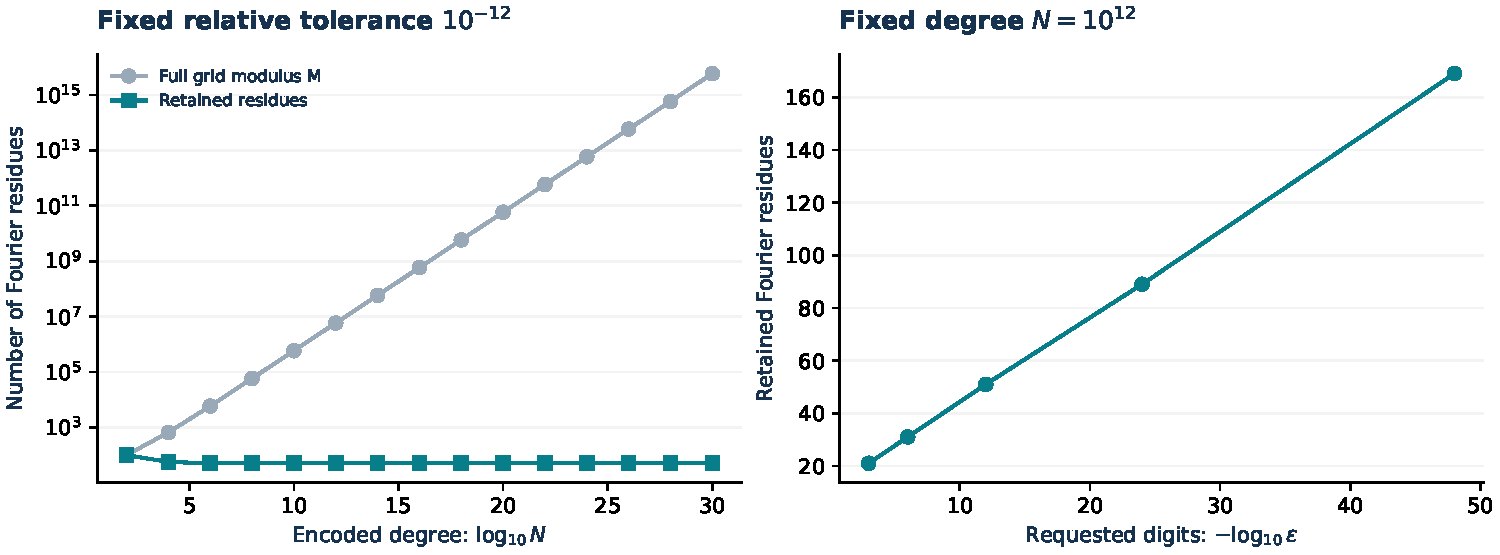
\includegraphics[width=0.94\textwidth]{figures/frequency_scaling.pdf}
\caption{Grid modulus and retained Fourier work for grouped binomial examples. The plot reports the actual certified algorithm's selected values. Its high-degree behavior illustrates the uniform frequency bound; elapsed time is not inferred from this plot.}\label{fig:frequencies}
\end{figure}}{}

\subsection{What the artifacts do and do not certify}

The ball intervals certify the reported numerical outputs, conditional on the documented arithmetic library. They are not Lean formalizations of the mathematical proofs. Exact rational enumeration provides a second implementation path for the small cases. The proof of the lazy-bit table sampler is included, while the supplied finite-support rational sampler provides a readable reference implementation rather than the claimed capacity-independent engineering realization. No runtime comparison with a fully optimized production implementation is claimed solely from operation counts.

\section{Limitations, possible failure modes, and extensions}\label{sec:limits}

\textbf{Accuracy notions.} The coefficient guarantee is relative. The individual conditional-marginal guarantee is additive. A very small marginal may consequently have a large relative error. Asking for simultaneous relative accuracy in all marginals requires a new analysis or a suitable extra tilt for each target.

\textbf{Masses and tails.} The main Fourier theorem computes a single atom. It does not by itself give the same uniform complexity for an entire tail probability. Tail inversion introduces a geometric or finite-sum kernel, whose interaction with the scale $\theta\sqrt V$ deserves separate treatment.

\textbf{Lattice structure.} The single central Fourier region comes from unit Bernoulli increments. With arbitrary integer weights, characteristic functions can have additional large peaks and support gaps. Copying the cutoff without treating those peaks is invalid. Similarly, a multivariate version needs covariance and lattice-volume control.

\textbf{Numerical scope.} The exact-real Newton count is proved independently of the conservative interval search used in the reference implementation. Ball arithmetic verifies finite calculations but can cost more than ordinary floating point. Powers with enormous multiplicities need guard bits of order $\log N$, even though their operation count is logarithmic in each multiplicity.

\textbf{Sampling scope.} The $\sqrt n$ bound counts independent proposals, not updates of a Markov chain. Each proposal requires up to $n-1$ coordinate variates. Exactness rests on exact or lazily certified comparisons. A standard floating-point inverse transform is insufficient to establish exact uniformity.

\textbf{Novelty scope.} The literature survey found the component techniques in established sources. The concrete improvements claimed here are the uniform relative coefficient theorem, its simultaneous/succinct consequences, and the uniform finite-margin PDC bound. Their priority would require a broader specialist review before publication. The mathematical proofs remain independently assessable regardless of that priority question.

\section{Further research questions and a proposed program}\label{sec:future}

\begin{enumerate}[label=\textbf{Q\arabic*.},leftmargin=3em]
\item \textbf{Optimal uniform proposal constant.} Determine the best constant $C$ such that a suitable common tilt in the one-coordinate PDC family always needs at most $(C+o(1))\sqrt n$ proposals. Equation~\eqref{eq:geomsharp} points to $\sqrt{2\pi}$ as a natural lower benchmark for this family. A sharper local atom inequality could close the gap introduced by entropy.

\item \textbf{Block completion and effective dimension.} Replace the single residual coordinate by a short block. Can one prove a proposal bound depending on an effective number of spread-out coordinates while retaining a cheap exact sampler inside the block? The data-dependent quantity in \eqref{eq:effective} suggests which columns should be grouped.

\item \textbf{Full lazy-bit implementation.} Implement the binary-recurrence inverse CDF and interval comparison procedures in Appendix~\ref{app:bits}, then establish an explicit near-linear dependence on the bit length of the margins. The present proof intentionally leaves the logarithmic exponent unoptimized.

\item \textbf{Uniform single-tail Fourier theorem.} Establish an analogue of Theorem~\ref{thm:sparse} for $\Prob(S\ge k)$ with $\BigO(\log(1/\varepsilon))$ product evaluations across the crossover from central to rare tails. The kernel, the central lower bound, and the scale $\theta\sqrt V$ should be analyzed together.

\item \textbf{Relative accuracy for every marginal.} Determine whether all inclusion and exclusion marginals can be computed to uniform relative accuracy with the same Fourier work, including nearly deterministic conditioned laws. The low-variance case is the likely obstruction to a direct extension of the present additive guarantee.

\item \textbf{Weighted and multivariate lattice sums.} Identify computable lattice conditions under which a bounded number of Fourier regions suffices. Seek complexity in the lattice index, covariance eigenvalues, and number of constraints, with explicit examples showing why each parameter is needed.

\item \textbf{Optimal accuracy dependence.} Is the logarithmic frequency count optimal for a clearly specified black-box product-evaluation model? Higher-order local expansions or other quadratures may improve constants or the dependence on extremely high precision; a matching lower bound would clarify the issue.

\item \textbf{Batched coefficient targets.} Several adjacent targets have nearby tilts. Develop a shared-contour or interpolation scheme that computes a block of coefficients while preserving relative certificates and compare its cost with full polynomial multiplication.

\item \textbf{Certified sampling of weighted fixed-size subsets.} Combine the coefficient oracle with sequential conditioning or lazy rejection to produce exact samples of weighted $k$-subsets. Analyze cumulative numerical work and avoid converting additive marginal approximations into an unsupported exactness claim.

\item \textbf{Formal verification and reproducible benchmarks.} Formalize the coarse-mean entropy lemma, local Chernoff estimate, and alias identity first. Separately benchmark an optimized implementation against ShiftConvolve and product-tree convolution on the same output tasks and accuracy requirements. These are concrete next steps toward publication-quality validation.
\end{enumerate}

\appendix
\section{Constructive details for exact random-bit sampling}\label{app:bits}

This appendix supplies the details behind Theorem~\ref{thm:tablebits}. Assume $0<r<T/2$; equality permits $q=1$ immediately. Truncation lowers the mean of a nonnegative geometric variable, so
$\E_q S\le nq/(1-q)$. At centering this implies
\begin{equation}\label{eq:qstarminimum}
 q_*\ge\frac{r}{n+r}\ge\frac1{n+1}.
\end{equation}

\subsection{A derivative bound that permits approximate comparisons}

For any decreasing mass function on $\{0,\ldots,c\}$ with mean $a$, one has $\Var(X)\ge a/3$. To prove this, represent it as a mixture of the uniform laws on $\{0,\ldots,K\}$, with mixture weights $(k+1)(p_k-p_{k+1})$. These weights sum to one. Then $\E K=2a$ and total variance gives
\[
 \Var(X)=\tfrac13\E K^2+\tfrac13a-a^2
 \ge\tfrac13a^2+\tfrac13a\ge a/3.
\]
Each tilted coordinate is decreasing, hence for $\mu(q)=\E_qS$,
\begin{equation}\label{eq:qderivative}
 \mu'(q)=\Var_q(S)/q\ge\mu(q)/3\qquad(0<q\le1).
\end{equation}

Choose a positive dyadic $h\le[64(n+1)T]^{-1}$ of $\BigO(B)$ bit length and put $\eta=h/32$. Maintain a bracket $[\ell,u]$ containing $q_*$, initially $[0,1]$. At its midpoint $v$, obtain $z$ with a certified error $\abs{z-\mu(v)}\le\eta$.
If $z+\eta<r$, replace $\ell$ by $v$; if $z-\eta>r$, replace $u$ by $v$. Otherwise return the dyadic $q=v-12\eta$. In that last case $\abs{\mu(v)-r}\le2\eta$, and between $v$ and $q_*$ the mean is at least $1/2$. Equation~\eqref{eq:qderivative} implies $\abs{v-q_*}\le12\eta$. Therefore $0\le q_*-q\le24\eta<h$. If instead the bracket width first reaches $h$, return $q=\ell$, which has the same one-sided error bound. Equation~\eqref{eq:qstarminimum} gives $q\ge1/[2(n+1)]$ and
\[
 \log(q_*/q)\le(q_*-q)/q\le2(n+1)h<1/T.
\]
There are $\BigO(B)$ midpoint evaluations.

\subsection{Evaluating means without expanded rational powers}

For $L$ terms define
$Z_L(q)=\sum_{j=0}^{L-1}q^j$ and $R_L(q)=\sum_{j=0}^{L-1}jq^j$.
Together with $Q_L=q^L$, the recurrences
\[
 Z_{2L}=Z_L(1+Q_L),\qquad
 R_{2L}=R_L(1+Q_L)+LQ_LZ_L,\qquad Q_{2L}=Q_L^2
\]
compute the sums by binary splitting; an odd length requires one extra term. Each coordinate mean is $R_{c_i+1}/Z_{c_i+1}$. All intermediate sums are nonnegative, $Z_L\ge1$, $Z_L\le T+1$, and $R_L\le T(T+1)/2$. Directed interval arithmetic therefore evaluates the mean to absolute error $\eta/n$ using polynomially many bits and operations in $B$.

A conservative justification uses $\BigO(B^2)$ working bits in addition to the requested absolute precision: the recursion has $\BigO(B)$ depth, its local derivative bounds are at most $2^{\BigO(B)}$, and hence an error budget of $2^{-\BigO(B^2)}$ controls all propagated errors. This is intentionally loose but sufficient. Exact expansion of $q^c$ would have a bit length proportional to $c$ and is avoided.

\subsection{Lazy uniform comparisons}

A lazy fair-bit uniform variable $U\in[0,1]$ is represented by a growing dyadic interval. To sample a truncated geometric coordinate, locate the smallest $k$ for which
\[
 U<F_c(k)=Z_{k+1}(q)/Z_{c+1}(q)
\]
by binary search over $0,\ldots,c$. Compute each threshold as a certified interval. If its interval intersects the current interval for $U$, reveal more bits and refine the threshold until the comparison is decided. Equality has probability zero and no unresolved comparison is rounded.

At accuracy $2^{-p}$, the uniforms within $\BigO(2^{-p})$ of any of the at most $c+1$ CDF thresholds have total probability at most $\BigO((c+1)2^{-p})$. After $\BigO(B)$ initial bits, the required additional precision therefore has a geometric tail. The $\BigO(B)$ binary-search comparisons and the binary-sum evaluations have expected $\operatorname{poly}(B)$ bit cost. The same $U$ is reused throughout one inverse-CDF search, yielding $\BigO(B)$ expected random bits for that coordinate.

Accepting with probability $q^b$ uses the same lazy comparison with a repeated-squaring enclosure. Its expected additional random-bit cost is constant and its numerical cost is polynomial in $B$. Independent trials have acceptance probability at least $1/(5\ee\sqrt n)$. Summing their costs gives the expected bounds in Theorem~\ref{thm:tablebits}; the geometric proposal tail also gives almost-sure termination.

\section{Audit trail and artifact guide}\label{app:artifacts}

The archive contains the complete source of this article, its compiled PDF, the coefficient implementation, its tests, the exact rational sampling reference and checks, generated numerical results, and the plotting/reproduction driver. The build instructions identify which computations certify numerical enclosures, which checks use exact rational arithmetic, and which theorem has a proof-level rather than fully engineered bit implementation. Numerical tables are generated from the saved experiment records rather than manually transcribed.

Primary-source provenance is recorded in the bibliography and in the accompanying source manifest. The manuscript uses public papers as literature context; it does not redistribute their full texts. The tests and independently reviewed derivations are evidence for this draft, and no external peer review or formal proof-assistant verification is asserted.

\begin{thebibliography}{99}
\bibitem{openai} OpenAI. \emph{Mathematics manuscript collection}. Repository README, overview, and manuscript map, accessed 8 October 2026. \url{https://github.com/openai/math}. In particular, catalogue families 115 and 130 motivated the algorithmic questions considered here.

\bibitem{plk} N. Peres, A. Lee, and U. Keich. \emph{Exactly computing the tail of the Poisson-binomial distribution}. ACM Transactions on Mathematical Software \textbf{47} (2021), Article 35. DOI: \href{https://doi.org/10.1145/3460774}{10.1145/3460774}. Inspected preprint: \url{https://arxiv.org/abs/2004.07429}.

\bibitem{dks} I. Diakonikolas, D. M. Kane, and A. Stewart. \emph{Optimal learning via the Fourier transform for sums of independent integer random variables}. Proceedings of the 29th Conference on Learning Theory, PMLR \textbf{49} (2016), 831--849. \url{https://proceedings.mlr.press/v49/diakonikolas16a.html}.

\bibitem{bornemann} F. Bornemann. \emph{Accuracy and stability of computing high-order derivatives of analytic functions by Cauchy integrals}. Foundations of Computational Mathematics \textbf{11} (2011), 1--63. DOI: \href{https://doi.org/10.1007/s10208-010-9075-z}{10.1007/s10208-010-9075-z}. Author preprint: \url{https://arxiv.org/abs/0910.1841}.

\bibitem{wk2017} D. Wilson and U. Keich. \emph{Accurate small tail probabilities of sums of iid lattice-valued random variables via FFT}. Journal of Computational and Graphical Statistics \textbf{26} (2017), 223--229. DOI: \href{https://doi.org/10.1080/10618600.2016.1276841}{10.1080/10618600.2016.1276841}.

\bibitem{wk2016} D. Wilson and U. Keich. \emph{Accurate pairwise convolutions of non-negative vectors via FFT}. Computational Statistics \& Data Analysis \textbf{101} (2016), 300--315. DOI: \href{https://doi.org/10.1016/j.csda.2016.03.010}{10.1016/j.csda.2016.03.010}.

\bibitem{dg} M. Dyer and C. Greenhill. \emph{Polynomial-time counting and sampling of two-rowed contingency tables}. Theoretical Computer Science \textbf{246} (2000), 265--278. DOI: \href{https://doi.org/10.1016/S0304-3975(99)00136-X}{10.1016/S0304-3975(99)00136-X}.

\bibitem{km} S. Kijima and T. Matsui. \emph{Polynomial time perfect sampling algorithm for two-rowed contingency tables}. Random Structures \& Algorithms \textbf{29} (2006), 243--256. Author report: \url{https://shuji-kijima.com/papers/METR2003-15.pdf}.

\bibitem{dz} S. DeSalvo and J. Y. Zhao. \emph{Random sampling of contingency tables via probabilistic divide-and-conquer}. Inspected version: arXiv:1507.00070v4, 29 February 2016. \url{https://arxiv.org/abs/1507.00070}. Published in Computational Statistics \textbf{35} (2020), 837--869. DOI: \href{https://doi.org/10.1007/s00180-019-00899-7}{10.1007/s00180-019-00899-7}.

\bibitem{brent} R. P. Brent. \emph{Fast multiple-precision evaluation of elementary functions}. Journal of the ACM \textbf{23} (1976), 242--251. DOI: \href{https://doi.org/10.1145/321941.321944}{10.1145/321941.321944}.

\bibitem{johansson} F. Johansson. \emph{Arb: efficient arbitrary-precision midpoint-radius interval arithmetic}. IEEE Transactions on Computers \textbf{66} (2017), 1281--1292. DOI: \href{https://doi.org/10.1109/TC.2017.2690633}{10.1109/TC.2017.2690633}. The implementation uses Arb/Acb through python-flint.
\end{thebibliography}
\end{document}
